\documentclass[11pt]{article}

\usepackage[a4paper,margin=1in]{geometry}
\usepackage{amsmath,amssymb}
\usepackage{booktabs}
\usepackage{graphicx}
\usepackage[colorlinks=true,linkcolor=blue,citecolor=blue,urlcolor=blue]{hyperref}
% lightweight unit macro (siunitx not available in this TeX install)
\newcommand{\SI}[2]{#1\,#2}
\newcommand{\si}[1]{#1}

\newcommand{\vx}{\mathbf{x}}
\newcommand{\vW}{\mathbf{W}}
\newcommand{\vg}{\mathbf{g}}
\newcommand{\vv}{\mathbf{v}}
\newcommand{\vu}{\mathbf{u}}
\newcommand{\vn}{\mathbf{n}}
\newcommand{\grad}{\nabla}
\newcommand{\Rp}{P_{\!R}}
\newcommand{\Ip}{P_{\!I}}

\title{Exact-gradient adaptation for AVC algorithm}
\author{Marco Falotico}
\date{\today}

\begin{document}
\maketitle

\begin{abstract}
The adaptive vibration cancellation (AVC) algorithm of Muradore, Pettazzi,
Fedrigo \& Clare (SPIE 8447-38) updates its state by a \emph{pseudo}-gradient:
it descends the squared prediction error while treating the regressor
$\vW$ as independent of the state, even though $\vW$ depends on the state
through the control parameters $\theta$. We derive the exact gradient,
including the dropped chain-rule term, in closed form. Two structural facts
follow analytically and are confirmed numerically: (i) even the exact
gradient leaves the plant-response parameters \emph{unobservable} from a
single tone (the update direction is confined to a two-dimensional
per-cycle subspace, so the averaged information matrix has rank two); and
(ii) applying the exact gradient to the \emph{disturbance} parameters
attenuates their update by a factor $\theta_{\min}/(|P|^2+\theta_{\min})$,
destroying the integral action that actually cancels the vibration. These
motivate a \emph{hybrid} update---exact gradient on the plant parameters,
pseudo-gradient (integral action) on the disturbance parameters---which we
implement and exercise in a closed-loop SPECULA single-conjugate AO
simulation. In a controlled comparison (identical loop, identical
atmosphere and vibration realisation, \emph{only} the state update
differing) the original pseudo-gradient with online plant adaptation
delivers \emph{no cancellation at all} ($+0.1$\,dB on the \SI{47}{Hz} tone
relative to the no-AVC baseline) while its plant estimate wanders
chaotically over three decades in magnitude and the full $\pm180^\circ$ in
phase, and its disturbance estimate grows without bound. The corrected
hybrid, from the same seeds, cancels the tone by $-48$ to $-59$\,dB and
reduces the mode-0 residual RMS by $94$--$96\%$. Its plant estimate
nonetheless makes only a bounded, \emph{radial} (magnitude-only)
adjustment---the phase never rotates toward the true value---an explicit
picture of the unobservability, and the reason a measured, frozen plant
remains the best-performing reference ($-63$\,dB).
\end{abstract}

\section{The algorithm}
\label{sec:alg}

Following the paper, a single AVC instance tracks one sinusoidal
disturbance at (angular) phase $\alpha(t)$. Its state collects the real and
imaginary parts of the plant frequency response and of the disturbance
quadratures,
\begin{equation}
  \vx = (x_1,x_2,x_3,x_4)^{\!\top} = (\Rp,\ \Ip,\ \lambda_c,\ \lambda_s)^{\!\top}.
\end{equation}
From $\vx$ it forms the control quadratures $\theta=(\theta_c,\theta_s)$
that would cancel the disturbance if $\vx$ were correct (their eq.~11),
\begin{equation}
  \theta_c = -\frac{x_1x_3-x_2x_4}{D},\qquad
  \theta_s = -\frac{x_1x_4+x_2x_3}{D},\qquad
  D = x_1^2+x_2^2+\epsilon,
  \label{eq:theta}
\end{equation}
where $\epsilon\ge 0$ is a regulariser on the otherwise singular
denominator, discussed in the next paragraph. With $c\equiv\cos\alpha$,
$s\equiv\sin\alpha$, the time-varying regressor (their eq.~9) is
\begin{equation}
  \vW(\alpha,\theta) =
  \begin{pmatrix}
    \theta_c\, c + \theta_s\, s\\
    \theta_s\, c - \theta_c\, s\\
    c\\ s
  \end{pmatrix},
  \label{eq:W}
\end{equation}
and the measurement model is $y = \vW^{\!\top}\vx$, an identity when $\vx$
holds the true plant and disturbance. Writing the prediction (equation)
error $e = \vW^{\!\top}\hat\vx - y$ and cost
$J=\tfrac12 e^2$, the paper updates (their eq.~10, discretised with step
$\mu = g_x T_s$)
\begin{equation}
  \hat\vx \leftarrow \hat\vx - \mu\, \vW\, e .
  \label{eq:pseudo}
\end{equation}

\paragraph{The regulariser $\epsilon$.}
The paper divides by $x_1^2+x_2^2$ exactly, i.e.\ $\epsilon=0$. That
denominator is the squared magnitude of the \emph{plant estimate}, so the
control gain \eqref{eq:theta} diverges whenever the estimate approaches the
origin---an event the update law does nothing to prevent. Implementations
therefore guard it: ESO's \texttt{updateAVC.m} freezes $\theta$ to $(1,0)$
whenever $x_1^2+x_2^2<10^{-2}$, a \emph{discontinuous} clamp. We use
instead the smooth equivalent $D=x_1^2+x_2^2+\epsilon$ with
$\epsilon=\theta_{\min}=10^{-2}$ by default (\texttt{theta\_min\_energy}
and \texttt{soft\_clamp} in the code), which bounds the gain by
$\sim\!1/\epsilon$ without introducing a switching boundary for the state
to chatter against.

Although $\epsilon$ is a numerical safeguard absent from the published
algorithm, it turns out to control the entire magnitude of the exact
gradient: every component of $\vg$ carries a factor $\epsilon$
(Secs.~\ref{sec:g3} and \ref{sec:radial}), and at $\epsilon=0$ the exact
gradient vanishes identically (Remark~\ref{rem:eps0}). It is therefore
worth tracking explicitly rather than treating as an implementation
detail.

\section{Exact differentiation}
\label{sec:exact}

Equation~\eqref{eq:pseudo} is \emph{not} the gradient of $J$. Because
$\vW=\vW(\theta(\hat\vx))$ depends on the estimate, the exact derivative of
the error is
\begin{equation}
  \frac{\partial e}{\partial x_i}
    = \frac{\partial (\vW^{\!\top}\vx)}{\partial x_i}
    = W_i + \sum_{j} \frac{\partial W_j}{\partial x_i}\, x_j
    = \big(\vW + J_{\!\vW}^{\top}\vx\big)_i,
  \qquad (J_{\!\vW})_{ji}=\frac{\partial W_j}{\partial x_i},
  \label{eq:dedx}
\end{equation}
($y$ is data, hence constant in $\hat\vx$ at the current step). The paper
keeps only $W_i$ and drops the chain-rule term $J_{\!\vW}^{\top}\vx$. The
\emph{exact} update descends along
\begin{equation}
  \vg \;=\; \vW + J_{\!\vW}^{\top}\vx .
  \label{eq:g}
\end{equation}

\paragraph{The Jacobian.}
Only $W_1,W_2$ depend on $\vx$ (through $\theta$); $W_3=c$, $W_4=s$ are
constant. Hence, using \eqref{eq:W},
$\partial W_1/\partial x_i = c\,\partial_i\theta_c + s\,\partial_i\theta_s$
and
$\partial W_2/\partial x_i = c\,\partial_i\theta_s - s\,\partial_i\theta_c$,
so the chain-rule term collapses to a two-term combination
\begin{equation}
  \big(J_{\!\vW}^{\top}\vx\big)_i
   = x_1\frac{\partial W_1}{\partial x_i} + x_2\frac{\partial W_2}{\partial x_i}
   = A\,\partial_i\theta_c + B\,\partial_i\theta_s,
  \qquad
  \begin{aligned}
    A &= x_1 c - x_2 s,\\
    B &= x_1 s + x_2 c,
  \end{aligned}
  \label{eq:AB}
\end{equation}
with the derivatives of \eqref{eq:theta} (writing $\partial_i\equiv\partial/\partial x_i$)
\begin{equation}
  \grad\theta_c = \frac1D\!
  \begin{pmatrix} -x_3-2x_1\theta_c\\ x_4-2x_2\theta_c\\ -x_1\\ x_2\end{pmatrix}\!,
  \qquad
  \grad\theta_s = \frac1D\!
  \begin{pmatrix} -x_4-2x_1\theta_s\\ -x_3-2x_2\theta_s\\ -x_2\\ -x_1\end{pmatrix}\!.
  \label{eq:gradtheta}
\end{equation}
Equations~\eqref{eq:g}--\eqref{eq:gradtheta} give $\vg$ analytically; they
agree with a finite-difference Jacobian to $\sim\!10^{-9}$ relative error,
and the resulting SPECULA object reproduces an independent NumPy reference
trajectory to $\sim\!2\times10^{-17}$.

\section{Two structural consequences}
\label{sec:consequences}

\subsection{The plant stays unobservable (rank-2 information)}
\label{sec:rank}

The question here is a concrete one: if the estimate $\hat\vx$ is wrong,
does the measurement notice? Directions in parameter space along which
$\hat\vx$ can be perturbed \emph{without changing the predicted output at
any phase} are invisible to any algorithm that only looks at that output,
no matter how it descends. We show that a two-dimensional family of such
directions always exists, and that it contains the plant.

\paragraph{Complex notation.}
The algebra becomes transparent in complex form. Collect the plant and the
disturbance into two complex numbers, and the control into a third,
\begin{equation}
  P = x_1+ix_2,\qquad \Lambda = x_3+ix_4,\qquad \vartheta=\theta_c+i\theta_s .
\end{equation}
Since $(x_1+ix_2)(x_3+ix_4)=(x_1x_3-x_2x_4)+i(x_1x_4+x_2x_3)$, the two
numerators of \eqref{eq:theta} are precisely the real and imaginary parts
of $P\Lambda$, so \eqref{eq:theta} is the single statement
\begin{equation}
  \vartheta \;=\; -\,\frac{P\,\Lambda}{D}
  \;\;\xrightarrow[\ \epsilon\to0\ ]{}\;\;
  -\,\frac{\Lambda}{\overline{P}} ,
  \qquad D=|P|^2+\epsilon .
  \label{eq:thetacomplex}
\end{equation}
That is the design intent made explicit: the control is the disturbance
divided by the plant, i.e.\ ``whatever, once pushed through the plant,
cancels $\Lambda$''.

\paragraph{The measurement sees only one complex number.}
Writing the regressor \eqref{eq:W} in the same notation and collecting the
$\cos\alpha$ and $\sin\alpha$ parts of $\vW^{\!\top}\vx$ gives, after a
one-line computation,
\begin{equation}
  \boxed{\;\vW^{\!\top}\vx \;=\; \mathrm{Re}(Z)\cos\alpha+\mathrm{Im}(Z)\sin\alpha,
  \qquad Z \;=\; \vartheta\,\overline{P}+\Lambda \;}
  \label{eq:Z}
\end{equation}
(verified numerically to machine precision). This is the crux. The model
output depends on the four parameters $(P,\Lambda)$ \emph{only} through the
single complex number $Z$ --- two real numbers. The map
$(P,\Lambda)\mapsto Z$ goes from $\mathbb{R}^4$ to $\mathbb{R}^2$; for a
given control $\vartheta$ it is linear in $(\overline{P},\Lambda)$, so its
kernel is exactly two-dimensional:
\begin{equation}
  \delta Z = \vartheta\,\overline{\delta P}+\delta\Lambda = 0
  \quad\Longleftrightarrow\quad
  \delta\Lambda = -\,\vartheta\,\overline{\delta P}\, .
  \label{eq:kernel}
\end{equation}
In words: \emph{any} change in the plant estimate can be exactly
compensated by a corresponding change in the disturbance estimate, leaving
every measurement, at every phase, for all time, bit-for-bit unchanged.
Choosing $\delta P=1$ and $\delta P=i$ gives the two null directions
explicitly,
\begin{equation}
  \vn_A=(1,\,0,\,-\theta_c,\,-\theta_s)^{\!\top},
  \qquad
  \vn_B=(0,\,1,\,-\theta_s,\,+\theta_c)^{\!\top},
  \label{eq:nulldirs}
\end{equation}
each carrying unit weight on a \emph{plant} axis. The ambiguity is
physical, not numerical: with a single tone one observes one complex
amplitude per cycle, while $P$ and $\Lambda$ together are two complex
unknowns. The problem is underdetermined by exactly a factor two, and
``how much does the plant scale my correction'' cannot be separated from
``how large is the disturbance''.

\paragraph{Why the exact gradient does not rescue this.}
Substituting \eqref{eq:AB} into \eqref{eq:g} and grouping the $c$ and $s$
terms,
\begin{equation}
  \vg = c\,\vv_1 + s\,\vv_2,\qquad
  \begin{aligned}
    \vv_1 &= \vu_1 + x_1\grad\theta_c + x_2\grad\theta_s,\\
    \vv_2 &= \vu_2 - x_2\grad\theta_c + x_1\grad\theta_s,
  \end{aligned}
  \label{eq:cvs}
\end{equation}
with $\vu_1=(\theta_c,\theta_s,1,0)^{\!\top}$ and
$\vu_2=(\theta_s,-\theta_c,0,1)^{\!\top}$ (so that
$\vW=c\,\vu_1+s\,\vu_2$). The vectors $\vv_1,\vv_2$ depend on the state but
\emph{not} on the phase $\alpha$. Hence, if the estimate is quasi-static
over one disturbance cycle (true for small step sizes, the regime of
interest), $\vg$ sweeps only the plane
$\mathrm{span}\{\vv_1,\vv_2\}$ and, averaging with
$\langle c^2\rangle=\langle s^2\rangle=\tfrac12$, $\langle cs\rangle=0$,
\begin{equation}
  \langle \vg\,\vg^{\!\top}\rangle
    = \tfrac12\big(\vv_1\vv_1^{\!\top}+\vv_2\vv_2^{\!\top}\big),
  \qquad \operatorname{rank}\le 2 .
  \label{eq:rank2}
\end{equation}
The information matrix is rank two whichever update direction is used:
correcting the gradient changes \emph{which} plane is explored, not the
fact that only a plane is explored. Numerically, with $\vartheta$ held
fixed the two remaining eigenvalues are zero to machine precision
($\sim\!10^{-14}$ against $\mathcal{O}(1)$).

\paragraph{A caveat, and why excitation does not help either.}
Equation~\eqref{eq:rank2} is exact for constant $\vartheta$. If $\vartheta$
varies in time the kernel \eqref{eq:kernel} rotates with it, and comparing
epochs with different $\vartheta$ \emph{would} in principle determine $P$:
from $Z^{(1)}-Z^{(2)}=(\vartheta^{(1)}-\vartheta^{(2)})\overline{P}$ at
constant $\Lambda$ one could solve for $\overline{P}$. This is exactly what
the offline probe measurement of the plant does, and it is why that
procedure works. It does \emph{not} rescue the online algorithm, for two
reasons: the instantaneous gradient carries no memory across epochs, so it
cannot form such differences; and $\vartheta$ is not an independent probe
but is slaved to the estimate through \eqref{eq:thetacomplex}, so it stops
varying precisely as the algorithm converges. Deliberately modulating the
\emph{disturbance} (amplitude or phase) leaves the two extra eigenvalues at
$\sim\!10^{-5}$ relative --- non-zero, but five orders below the observable
pair and useless on any practical timescale. Observability must come from
the command side, not the disturbance side.

\subsection{The exact gradient annihilates the disturbance drive}
\label{sec:g3}

For the disturbance components the chain-rule term nearly cancels the
direct term. Using $\partial\theta_c/\partial x_3=-x_1/D$,
$\partial\theta_s/\partial x_3=-x_2/D$ in \eqref{eq:AB},
\begin{equation}
  \big(J_{\!\vW}^{\top}\vx\big)_3
    = -\frac{A x_1 + B x_2}{D}
    = -\frac{(x_1^2+x_2^2)}{D}\,c,
\end{equation}
so that
\begin{equation}
  \boxed{\,g_3 = c - \frac{x_1^2+x_2^2}{D}\,c
        = c\,\frac{\epsilon}{D}
        = \cos\alpha\;\frac{\theta_{\min}}{|P|^2+\theta_{\min}}\,,}
  \qquad
  g_4 = \sin\alpha\;\frac{\theta_{\min}}{|P|^2+\theta_{\min}} .
  \label{eq:g3}
\end{equation}
(Verified to machine precision.) The exact-gradient disturbance drive is
the pseudo-gradient $(\cos\alpha,\sin\alpha)$ \emph{attenuated by
$\theta_{\min}/|P|^2$}: with $\theta_{\min}=10^{-2}$ and $|P|^2\!\sim\!52$
in the demo this is $\sim\!2\times10^{-4}$, i.e.\ the disturbance update is
effectively switched off.

The reason is structural, not numerical. The control
$\theta=-\lambda_{\text{est}}/P$ is \emph{designed} so that raising the
disturbance estimate raises the cancelling control by the same amount;
increasing $\lambda_{\text{est}}$ feeds a direct term ($+c\,\delta\lambda$
in $\vW^{\!\top}\vx$) and an indirect term through $\theta$
($-c\,\delta\lambda$) that almost annihilate. The chain-rule term is
exactly this indirect path. But minimising the equation error is the
\emph{wrong} objective for the disturbance: what we want is to drive the
\emph{physical residual} $y$ to zero, and there the pseudo-gradient is
exactly right. With the plant fixed, \eqref{eq:pseudo} restricted to
$x_3,x_4$ reads
\begin{equation}
  x_3 \leftarrow x_3 - \mu\,\cos\alpha\; e
  \quad\Longrightarrow\quad
  \frac{\mathrm d\lambda_{\text{est},c}}{\mathrm dt}
    \propto -\big(\lambda_{\text{est},c}-\lambda_c\big),
\end{equation}
i.e.\ a stable \emph{integral controller} that drives
$\lambda_{\text{est}}\!\to\!\lambda$ and hence $y\!\to\!0$. The disturbance
sub-problem is a well-posed linear regression against the persistently
exciting, observable regressor $(\cos\alpha,\sin\alpha)$; the plain
correlation is the correct estimator, and the chain-rule term must
\emph{not} be added.

\subsection{The exact plant update is radial, and of order $\epsilon$}
\label{sec:radial}

The same collapse happens on the plant side, in a more striking way.
Carrying the complex notation of Sec.~\ref{sec:rank} through
\eqref{eq:AB}--\eqref{eq:gradtheta} (using $A+iB=Pe^{i\alpha}$,
$\vartheta=-P\Lambda/D$, and $\Lambda e^{-i\alpha}+\overline{\Lambda}e^{i\alpha}=2\mathrm{Re}(\overline{\Lambda}e^{i\alpha})$)
the two plant components of the exact gradient collapse to the closed form
\begin{equation}
  \boxed{\;g_1+i\,g_2 \;=\; -\,2\,\mathcal{R}\,\frac{\epsilon}{D^{2}}\;P,
  \qquad \mathcal{R}\equiv\mathrm{Re}\!\left(\overline{\Lambda}\,e^{i\alpha}\right)\in\mathbb{R}\;}
  \label{eq:gplant}
\end{equation}
(verified to machine precision for several $\epsilon$). Two consequences,
both directly visible in the closed-loop runs of Sec.~\ref{sec:demo}:

\begin{itemize}\itemsep2pt
  \item \textbf{The update is exactly radial.} $g_1+ig_2$ is a
    \emph{real} multiple of $P$: the exact plant update can only lengthen
    or shorten the plant estimate, never rotate it. The phase $\arg P$ is a
    conserved quantity of the exact plant update. Numerically the cross
    product $g_1x_2-g_2x_1$ vanishes to $\sim\!10^{-13}$ relative, whereas
    for the pseudo-gradient the same quantity is of order unity---which is
    why the original algorithm's plant phase wanders over the full
    $\pm180^\circ$ (Fig.~\ref{fig:cmp}c) while the hybrid's sits exactly at
    its seed (Fig.~\ref{fig:tscale}). What looked empirically like ``the
    update cannot rotate $\arg P$'' is a theorem.
  \item \textbf{The update is $\mathcal{O}(\epsilon)$.} It is proportional
    to the regulariser $\epsilon=\theta_{\min}$ of \eqref{eq:theta}. With
    $\epsilon=0$ --- the paper's formula --- the exact gradient does not
    move the plant estimate \emph{at all}.
\end{itemize}

\paragraph{Why both components are $\mathcal{O}(\epsilon)$: the prediction is $\mathcal{O}(\epsilon)$.}
Equations~\eqref{eq:g3} and \eqref{eq:gplant} share the factor $\epsilon$
for one reason. Substituting the slaved control
\eqref{eq:thetacomplex} into \eqref{eq:Z} with $\vx=\hat\vx$,
\begin{equation}
  \hat Z=\vartheta\overline{\hat P}+\hat\Lambda
        =-\frac{\hat P\hat\Lambda}{D}\overline{\hat P}+\hat\Lambda
        =\hat\Lambda\Big(1-\frac{|\hat P|^{2}}{D}\Big)
        =\hat\Lambda\,\frac{\epsilon}{D}\;\xrightarrow[\ \epsilon\to0\ ]{}\;0 .
  \label{eq:Zhat}
\end{equation}
The predicted output is identically zero when $\epsilon=0$: by
construction, the control $\vartheta$ is the one that cancels
$\hat\Lambda$, so the model predicts perfect cancellation of its own
estimate. Consequently the prediction error is simply
$e=\vW^{\!\top}\hat\vx-y\simeq-y$, the negated physical residual, and the
exact gradient---the derivative of a quantity that is identically
zero---is itself $\mathcal{O}(\epsilon)$.

\begin{samepage}
\paragraph{Remark (the $\epsilon\to0$ collapse).}
\label{rem:eps0}
Taking the limit in \eqref{eq:g3} and \eqref{eq:gplant} simultaneously,
\begin{equation}
  \epsilon=0
  \quad\Longrightarrow\quad
  \vW^{\!\top}\hat\vx\equiv0\ \ \text{for every }\hat\vx
  \quad\Longrightarrow\quad
  J=\tfrac12\big(\vW^{\!\top}\hat\vx-y\big)^2=\tfrac12y^2
  \quad\Longrightarrow\quad
  \vg\equiv\mathbf{0}.
\end{equation}
With the paper's exact formula, the cost being minimised \emph{does not
depend on the parameters being optimised at all}: $\theta$ is constructed
to cancel $\hat\Lambda$, so the model always predicts perfect
cancellation of its own estimate, whatever that estimate is. A cost
independent of its arguments has zero gradient, and ``exact gradient
descent'' on it is a no-op. Numerically, at $\epsilon=0$ we measure
$\|\vg\|\sim4\times10^{-15}$ (machine zero) while $\|\vW\|\sim20$--$40$.
\end{samepage}

This is the sharpest statement of the paper's ``error'': the exact gradient
of the equation error is not merely a poor update, it is (up to the
regulariser) \emph{no update}. The pseudo-gradient is therefore not an
approximation to the exact gradient but a different, useful object---the
correlation of the physical residual with the regressor, i.e.\
LMS/integral action. It also explains, retrospectively, the
\texttt{full exact} row of Table~\ref{tab:cmp}: with both halves receiving
$\mathcal{O}(\epsilon)$ drives, the algorithm barely adapts at all, the
disturbance estimate never leaves its initial value, and no cancellation
occurs. By the same token, the modest plant adaptation that the hybrid
\emph{does} perform exists only by virtue of $\epsilon\neq0$: it is an
artefact of the safeguard, not of the algorithm as published.

\subsection{The hybrid update}
Sections~\ref{sec:rank}--\ref{sec:radial} motivate matching each half of the
state to its correct objective:
\begin{equation}
  \hat x_{1,2}\leftarrow \hat x_{1,2}-\mu\,c_{\!p}\,g_{1,2}\,e
  \quad(\text{exact}),\qquad
  \hat x_{3,4}\leftarrow \hat x_{3,4}-\mu\,W_{3,4}\,e
  \quad(\text{pseudo / integral}),
  \label{eq:hybrid}
\end{equation}
implemented as \texttt{exact\_gradient:\ plant} in the SPECULA
\texttt{AVC} object ($c_{\!p}$ is the plant-update damping constant
\texttt{c}). This gives the plant a true, non-diverging descent direction
while leaving the disturbance integrator intact.

\subsection{Why the plant update needs damping ($c_{\!p}$)}
\label{sec:damp}

The plant components need their own, much smaller step size. There are two
distinct reasons, one for each update variant, and it is worth separating
them because they behave differently.

\paragraph{(i) Pseudo-gradient: the loop gain grows as the canceller works.}
For a gradient step $\hat\vx\leftarrow\hat\vx-\mu M\vg\,e$ with
$M=\mathrm{diag}(c_{\!p},c_{\!p},1,1)$, linearising about a stationary
point gives $\delta\vx\leftarrow(I-\mu M\langle\vg\vg^{\!\top}\rangle)\delta\vx$,
so stability requires the eigenvalues of
$\mu M\langle\vg\vg^{\!\top}\rangle$ to lie in $(0,2)$. For the
pseudo-gradient this is computable in closed form: from
$\vW=c\,\vu_1+s\,\vu_2$ with
$\vu_1\cdot\vu_2=0$ and $|\vu_1|^2=|\vu_2|^2=|\vartheta|^2+1$,
\begin{equation}
  \langle\vW\vW^{\!\top}\rangle=\tfrac12\big(|\vartheta|^{2}+1\big)\,\Pi,
  \qquad
  \lambda_{\max}=\tfrac12\big(|\vartheta|^{2}+1\big),
  \label{eq:lmax}
\end{equation}
with $\Pi$ the projector onto $\mathrm{span}\{\vu_1,\vu_2\}$ (verified
numerically: the spectrum is $\{\lambda_{\max},\lambda_{\max},0,0\}$ to
machine precision). Because $|\vartheta|\!\gg\!1$ in practice, that
subspace lies almost entirely along the plant axes, so the binding
constraint is the plant one:
\begin{equation}
  \mu\,c_{\!p}\,\tfrac12\big(|\vartheta|^{2}+1\big)<2
  \qquad\Longleftrightarrow\qquad
  c_{\!p}\;<\;\frac{4}{g_xT_s\big(|\vartheta|^{2}+1\big)} .
  \label{eq:cpbound}
\end{equation}
The essential point is \emph{not} the constant but the scaling. By
\eqref{eq:thetacomplex}, $|\vartheta|=|\hat\Lambda|/|\hat P|$ grows from
$0$ at start-up (no correction yet) to a large value once the canceller has
built up its correction --- in the demo $|\vartheta|\!\approx\!82$, i.e.\
$|\vartheta|^2+1\approx6.9\times10^{3}$. \textbf{The plant-loop gain
therefore grows by orders of magnitude \emph{as cancellation improves}}:
a $c_{\!p}$ that is perfectly safe during the first transient can violate
\eqref{eq:cpbound} later, when the algorithm is working well. This is a
genuine trap, and it is one plausible reading of why the published
algorithm can appear stable in short tests and diverge in long ones. With
the demo numbers ($g_x=3$, $T_s=\SI{1}{ms}$), \eqref{eq:cpbound} gives
$c_{\!p}<0.19$.

\paragraph{(ii) Exact/hybrid gradient: a state-dependent blow-up near $|P|\to0$.}
For the hybrid the plant drive is \eqref{eq:gplant} rather than $\vW$, and
its magnitude is
\begin{equation}
  |g_1+ig_2| \;=\; 2|\mathcal{R}|\,\frac{\epsilon\,|P|}{D^{2}},
  \qquad D=|P|^{2}+\epsilon .
\end{equation}
This is small when $|P|^{2}\!\gg\!\epsilon$ (the $\mathcal{O}(\epsilon)$
regime of Sec.~\ref{sec:radial}) but \emph{grows} as $|P|$ shrinks, peaking
near $|P|^2\!\sim\!\epsilon$ where it behaves like $2|\mathcal{R}|/(\epsilon^{1/2})$
--- larger by $\sim\!1/\epsilon$ than in the well-conditioned regime. Since
the update is radial, a shrinking $|P|$ increases its own update gain: the
mechanism is a state-dependent runaway rather than a fixed-gain
instability, and $c_{\!p}$ is what keeps the trajectory out of it.

\paragraph{Practical determination.}
Equation~\eqref{eq:cpbound} is derived for a delay-free, noise-free loop
and should be treated as an order-of-magnitude guide, not a threshold: the
real loop adds three frames of delay and measurement noise, both of which
tighten it. The gap is easily seen --- in the idealised (delay-free) model
the hybrid remains bounded even at $c_{\!p}=1$, whereas in the closed loop
$c_{\!p}=1$ diverges. In practice $c_{\!p}$ is set empirically; the sweep
below (closed loop, $g_x=3$) shows a clear threshold between $0.1$ and $1$,
consistent with the $0.19$ predicted by \eqref{eq:cpbound}.

\begin{table}[h]
  \centering
  \begin{tabular}{lll}
    \toprule
    $c_{\!p}$ & plant estimate $|x_1{+}ix_2|$ & \SI{47}{Hz} residual\\
    \midrule
    $1.0$    & diverges ($\to\!309$)              & \SI{470}{nm} (no cancellation)\\
    $0.1$    & $7.22\!\to\!6.36$, settles         & \textbf{\SI{2}{nm}}\\
    $0.01$   & $7.22\!\to\!7.13$                  & \SI{11}{nm}\\
    $0.001$  & essentially frozen                 & \SI{12}{nm}\\
    \bottomrule
  \end{tabular}
  \caption{Empirical determination of the plant-update damping in the
  closed loop (hybrid update, $g_x=3$). Too large diverges; too small
  reduces to the frozen-plant case. Predicted bound
  \eqref{eq:cpbound}: $c_{\!p}<0.19$.}
  \label{tab:cp}
\end{table}

\section{Idealised experiments}
\label{sec:ideal}

These use only the algorithm's equations (no AO loop, no delay, no noise,
known fixed frequency, measurement $y=\vW^{\!\top}\vx_\star$), so any
pathology is intrinsic to the algorithm.

\paragraph{Observability (\texttt{avc\_observability\_check.py}).}
With $\theta$ frozen at the truth the update is linear, and the averaged
information matrix has eigenvalues
$(1.777,\,1.777,\,1.8\!\times\!10^{-14},\,1.8\!\times\!10^{-14})$: two
non-zero, two zero to machine precision (rank 2). The observable component
of the estimate error is driven to $\sim\!10^{-13}$ while the unobservable
component is frozen at its initial value. Seeding the plant at the true
value and running the full (non-linear) update, the estimate nonetheless
diverges (magnitude $0.55\!\to\!$ thousands): unobservable drift plus the
$1/(x_1^2+x_2^2)$ feedback. Freezing the plant and adapting only
$x_3,x_4$ recovers the true disturbance exactly
($(1000.000,-0.000)$ vs.\ $(1000,0)$; error $\sim\!2\times10^{-6}$).

\paragraph{Pseudo vs.\ exact (\texttt{avc\_chainrule\_check.py}).}
Table~\ref{tab:chain} contrasts the two update directions from a slightly
wrong plant seed. The pseudo-gradient \emph{actively wanders}; the exact
gradient \emph{settles} (a true gradient vanishes on the zero-error
manifold) but at a wrong value---neither identifies the plant, consistent
with Sec.~\ref{sec:rank}.

\begin{table}[h]
  \centering
  \begin{tabular}{lccc}
    \toprule
    update & final plant error & eig$\langle\vg\vg^{\!\top}\rangle$ & plant identified?\\
    \midrule
    pseudo (chain term dropped) & $0.265$ (drifts up from $0.071$) & $[1.73,1.73,\!\sim\!0,\!\sim\!0]$ & no (wanders)\\
    exact (chain term kept)     & $0.063$ (settles)               & $[\!\sim\!0,\!\sim\!0,\!\sim\!0,\!\sim\!0]$ & no (wrong value)\\
    \bottomrule
  \end{tabular}
  \caption{Idealised single-tone adaptation; small amplitude for a stable step size.}
  \label{tab:chain}
\end{table}

\section{Closed-loop SPECULA demonstration}
\label{sec:demo}

The full demo is a single-conjugate AO loop (\SI{64}{px} pupil, $8\times8$
Shack--Hartmann, 40 Zernike modes, \SI{1}{kHz}) with a standard integrator
(gain $0.5$, 2-frame delay) on all modes, a first-order \SI{80}{Hz}
actuator low-pass, and a \SI{47}{Hz} tip vibration. AVC runs in parallel on
mode~0, its command summed with the integrator's.

\paragraph{Where AVC is useful.}
The integrator rejects low frequencies but, above its bandwidth, the
sensitivity $|S|=|1/(1+H_{\text{OL}})|$ exceeds unity (waterbed). The
measured/analytic rejection is $-38,-24,-17,-9$\,dB at $1,5,10,20$\,Hz but
strongly positive at \SI{47}{Hz}: the injected \SI{120}{nm} tone emerges as
a \SI{891}{nm} residual, an amplification of $7.4\times$ ($+17.4$\,dB).
This is precisely where a narrow-band canceller earns its place---the main
controller actively makes the disturbance worse and cannot be retuned to
fix it without sacrificing low-frequency performance.

\subsection{Controlled comparison: original vs.\ corrected update}
\label{sec:cmp}

To isolate the effect of the gradient alone, six \SI{10}{s} runs were
performed that are \emph{identical in every respect}---same seeded
atmosphere, same vibration realisation, same loop, same
$g_x=3$, $g_\omega=0.2$, $c_{\!p}=0.1$, same \SI{45}{Hz} initial frequency
guess---differing \emph{only} in the state-update rule and the plant seed.
Two seeds are used: the measured closed-loop value
($|P|=7.22\,\angle\,169.5^\circ$, ``correct'') and a deliberately wrong one
($|P|=1.41\,\angle\,135^\circ$). Results are collected in
Table~\ref{tab:cmp} and Fig.~\ref{fig:cmp}; steady-state statistics are
taken over the second half of each run.

\begin{table}[h]
  \centering
  \small
  \begin{tabular}{llrrrrr}
    \toprule
    update & plant seed & mode-0 RMS & all-mode RMS & \SI{47}{Hz} amp. & vs.\ base & final $|x_1{+}ix_2|$\\
    \midrule
    none (baseline)   & ---     & \SI{630.4}{nm} & \SI{99.9}{nm} & \SI{891}{nm} & ---            & ---\\
    \midrule
    ORIGINAL pseudo   & wrong   & \SI{640.7}{nm} & \SI{101.5}{nm}& \SI{898}{nm} & $+0.1$\,dB     & $205$ (wandering)\\
    ORIGINAL pseudo   & correct & \SI{639.6}{nm} & \SI{101.3}{nm}& \SI{896}{nm} & $+0.0$\,dB     & $64$ (wandering)\\
    \midrule
    CORRECTED hybrid  & wrong   & \SI{36.5}{nm}  & \SI{7.3}{nm}  & \SI{3.5}{nm} & $\mathbf{-48.2}$\,dB & $13.8$ (settled)\\
    CORRECTED hybrid  & correct & \SI{27.5}{nm}  & \SI{6.2}{nm}  & \SI{1.0}{nm} & $\mathbf{-58.9}$\,dB & $4.0$ (settled)\\
    \midrule
    frozen plant      & correct & \SI{26.5}{nm}  & \SI{6.1}{nm}  & \SI{0.6}{nm} & $-63.0$\,dB    & $7.22$ (fixed)\\
    \bottomrule
  \end{tabular}
  \caption{Controlled comparison; only the state update and plant seed
  differ. The original pseudo-gradient with online plant adaptation
  provides no cancellation whatsoever (it is marginally \emph{worse} than
  doing nothing); the corrected hybrid cancels by $48$--$59$\,dB. A
  measured, frozen plant remains the best performer.}
  \label{tab:cmp}
\end{table}

\begin{figure}[htbp]
  \centering
  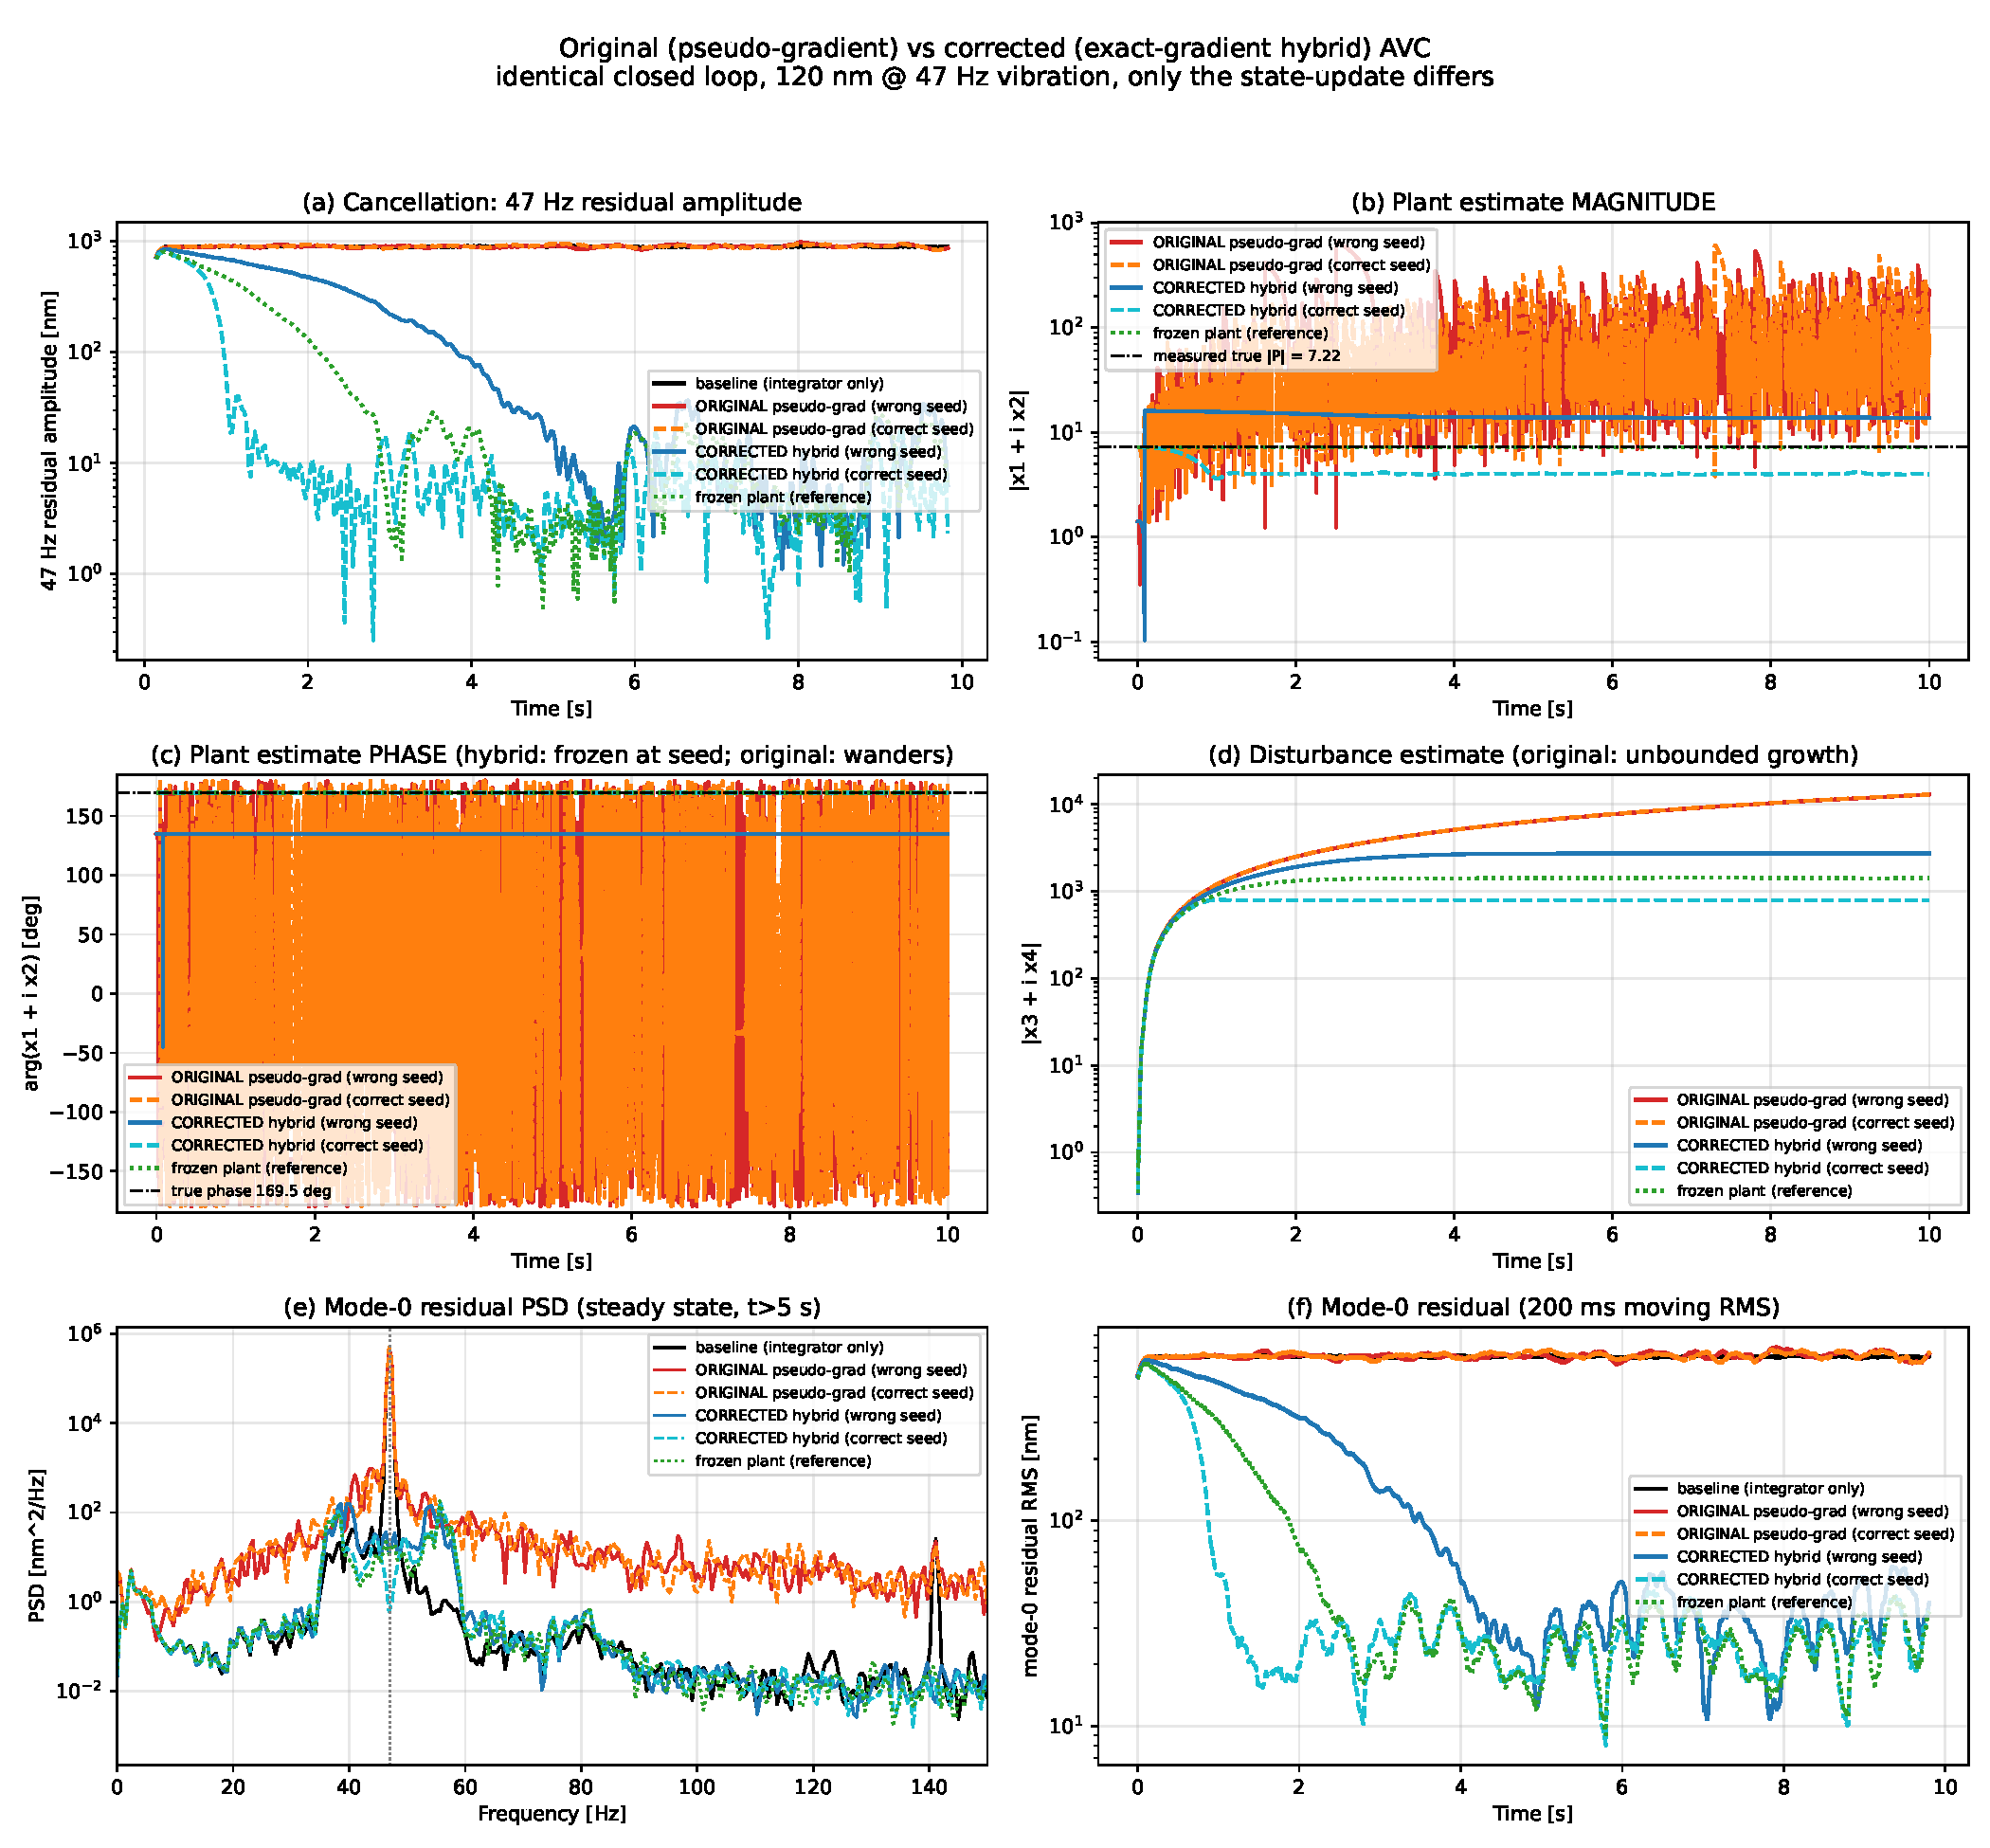
\includegraphics[width=\textwidth]{avc_gradient_comparison.pdf}
  \caption{Original vs.\ corrected AVC under identical conditions.
  (a) the two ORIGINAL traces sit on the baseline---no cancellation---while
  the corrected hybrid and the frozen reference fall by 2--3 decades;
  (b),(c) the original plant estimate wanders over three decades in
  magnitude and fills the full $\pm180^\circ$ in phase, whereas the hybrid
  settles and holds its seed phase exactly;
  (d) the original disturbance estimate grows without bound
  ($\to\!1.3\times10^{4}$ and still rising at \SI{10}{s}) while the hybrid
  plateaus; (e) in the steady-state PSD the original \emph{enlarges} the
  \SI{47}{Hz} peak and raises the broadband floor; (f) mode-0 residual.}
  \label{fig:cmp}
\end{figure}

Three observations follow.
\begin{itemize}\itemsep2pt
  \item \textbf{The original update fails outright when the plant is
    adapted online}, and the failure is insensitive to the seed: starting
    from the exactly measured plant is no better than starting from a
    deliberately wrong one ($+0.0$ vs.\ $+0.1$\,dB). This is the signature
    of a divergence driven by the update law itself, not of a poor
    initialisation. Panel~(e) shows it is in fact mildly harmful: the
    \SI{47}{Hz} peak is \emph{larger} than the baseline and the broadband
    floor is raised, because a large, wrongly-phased correction is being
    injected.
  \item \textbf{The corrected hybrid works from either seed}, differing
    only in convergence time and final depth ($-48.2$\,dB from the wrong
    seed, $-58.9$\,dB from the correct one; cf.\ panel~(a), where the
    wrong-seed trace takes ${\sim}\SI{5}{s}$ rather than ${\sim}\SI{2}{s}$
    to converge). Its disturbance estimate plateaus rather than diverging.
  \item \textbf{Neither variant identifies the plant.} The hybrid's
    estimate settles at $|P|=4.0$ (correct seed) or $13.8$ (wrong seed),
    neither being the true $7.22$, and panel~(c) shows the phase pinned at
    whatever value it was seeded with. Cancellation is nevertheless
    excellent, because the disturbance integrator compensates for any
    stable, correctly-\emph{phased} plant estimate. The residual gap to the
    frozen reference ($-58.9$ vs.\ $-63.0$\,dB) is the price of letting the
    magnitude drift at all.
\end{itemize}

\subsection{Convergence timescales from a wrong seed}
The wrong-seed hybrid run of Table~\ref{tab:cmp} separates three distinct
timescales, shown in Fig.~\ref{fig:tscale}:
\begin{itemize}\itemsep2pt
  \item \textbf{Plant magnitude} rescales $1.41\!\to\!13.8$ within a
    fraction of a second, then settles---\emph{not} at the true $7.22$.
  \item \textbf{Plant phase} is frozen at the seed $135.000^\circ$ (to
    three decimals, over \SI{10}{s}): the hybrid update is effectively
    \emph{radial}, adjusting $|P|$ but never $\arg P$. This is the rank
    deficiency of Sec.~\ref{sec:rank} made directly visible.
  \item \textbf{Cancellation} nonetheless converges, on the
    disturbance-loop timescale set by $g_x$ (${\sim}\SI{3.9}{s}$ to a
    $10\times$ reduction): the \SI{47}{Hz} residual falls
    $891\!\to\!6.8$\,nm, because the integral loop on $x_3,x_4$ compensates
    for whatever stable, correctly-phased plant estimate it is handed.
\end{itemize}
The frequency loop is a fourth, independent timescale: it locks from the
wrong \SI{45}{Hz} guess to \SI{46.98}{Hz} with \SI{0.02}{Hz} jitter, driven
by the quadrature error $\sin\alpha\,e$ and requiring no plant knowledge at
all---which is why frequency tracking succeeded throughout this study even
when plant estimation did not.

\begin{figure}[htbp]
  \centering
  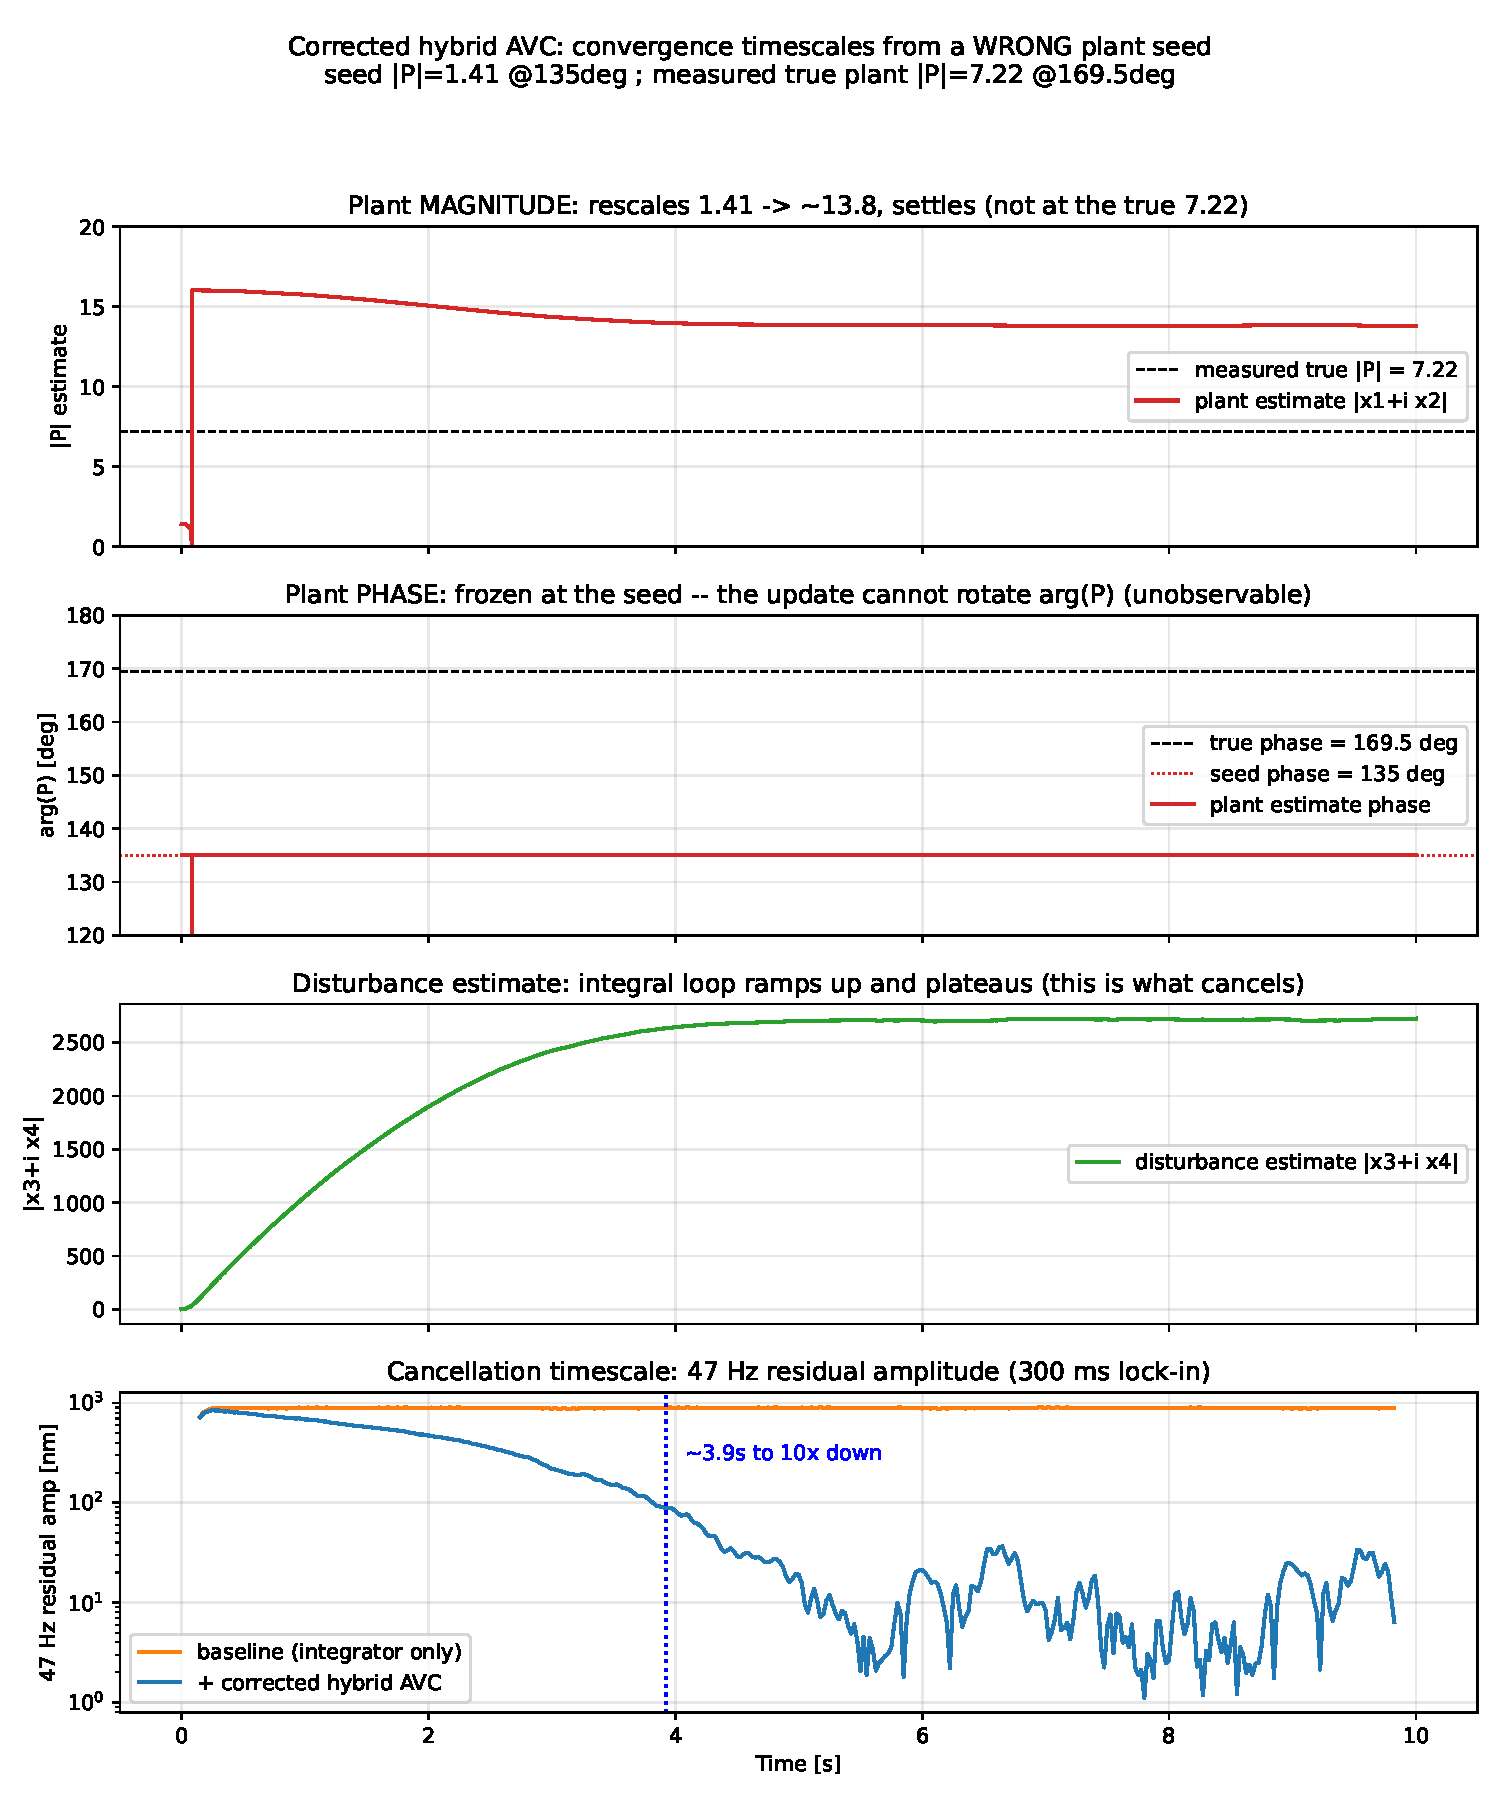
\includegraphics[height=0.80\textheight]{avc_convergence_timescales.pdf}
  \caption{Corrected hybrid AVC from a wrong plant seed. Top to bottom:
  plant magnitude (rescales, misses the true value); plant phase (frozen at
  the seed---no rotation, unobservable); disturbance estimate (the integral
  ramp that does the cancelling); \SI{47}{Hz} residual amplitude, baseline
  vs.\ AVC, ${\sim}\SI{3.9}{s}$ to $10\times$ down.}
  \label{fig:tscale}
\end{figure}

\section{Discussion}
\label{sec:disc}

The two halves of the AVC state require different objectives, and the
hybrid assigns each its correct one. The \emph{disturbance} parameters form
an observable linear regression whose goal is to null the physical
residual; the pseudo-gradient is a certainty-equivalence integral
controller that does exactly this, and the exact gradient sabotages it via
\eqref{eq:g3}. The \emph{plant} parameters are the nonlinear,
self-referential, single-tone-unobservable part where the pseudo-gradient's
neglect of $\partial\vW/\partial\vx$ causes active divergence; the exact
gradient supplies a genuine descent direction that merely settles.
Equivalently, the hybrid is a filtered-X-LMS structure: an LMS/integral
canceller whose reference is filtered by the plant estimate (through
$\theta$), with the plant adapted on a separate, damped, stabilised path
and never fed the term that would break the canceller.

Three practical corollaries follow. First, \textbf{the published update law
must not be run with online plant adaptation}: Table~\ref{tab:cmp} shows it
then yields no cancellation at all, and does so regardless of how well the
plant is initialised---the failure is in the update, not the
initialisation. The paper's own practice (seeding with approximate
closed-loop plant values and relying on fast error nulling) is much closer
to our ``frozen'' configuration, which is also the best performer here;
read that way, our results are consistent with the paper's reported
success rather than contradicting it.

Second, \textbf{the plant is not identifiable online from a single tone}.
Seed its \emph{phase} approximately correctly---from a calibration, a probe
measurement, or the analytic model---because no variant of the update can
rotate it; the \emph{magnitude} is forgiving, since the disturbance
integrator absorbs a scale error.

Third, for a static plant the simplest robust choice remains a frozen,
measured plant ($-63.0$\,dB here). The corrected hybrid costs
${\sim}4$\,dB relative to that but adds the ability to track slow plant
changes without the runaway; it is the appropriate choice when the plant
drifts (thermal or elevation-dependent effects over a night) and
recalibration is impractical.

\paragraph{Reproducibility.}
Derivation checks: \texttt{avc\_chainrule\_check.py} (finite-difference and
reference-trajectory validation of the Jacobian and of
Eq.~\eqref{eq:g3}), \texttt{avc\_observability\_check.py} (rank-2
information matrix, drift). Closed-loop configurations:
\texttt{params\_scao\_avc\_full\_demo.yml} (AVC; the update variant is
selected by the \texttt{adapt\_plant} and \texttt{exact\_gradient} keys of
the \texttt{avc:} block), \texttt{params\_scao\_vibration\_baseline.yml}
(integrator only), \texttt{params\_measure\_plant.yml} (closed-loop plant
measurement by probe injection and lock-in). The six runs of
Table~\ref{tab:cmp} share the atmospheric seed (\texttt{AtmoEvolution}
\texttt{seed}$=1$), so they differ only in the AVC update; per-run
statistics and Figs.~\ref{fig:cmp}--\ref{fig:tscale} are produced by the
comparison scripts described in \texttt{README.md}, and the standard
five-panel diagnostic by \texttt{analyze\_results.py}.

\paragraph{Software.}
The update variants are implemented in
\texttt{specula/processing\_objects/avc.py}: \texttt{adapt\_plant}
(freeze/adapt $x_1,x_2$), \texttt{exact\_gradient} $\in$
\{\texttt{false}, \texttt{'plant'}, \texttt{'full'}\} (which components
receive the chain-rule term), and \texttt{soft\_clamp} (the $\epsilon$
regulariser of Eq.~\eqref{eq:theta}). The defaults
(\texttt{exact\_gradient:\ false}, \texttt{adapt\_plant:\ true},
\texttt{soft\_clamp:\ false}) reproduce the published algorithm bit-for-bit
and are covered by a Matlab-reference regression test.

\appendix
\section{Step-by-step computation of the Jacobian}
\label{app:jac}

This appendix expands Sec.~\ref{sec:exact} in full so the algebra can be
checked line by line. Every entry below was verified against a
finite-difference Jacobian (agreement $\sim\!10^{-8}$).

\paragraph{Notation.}
With $c\equiv\cos\alpha$, $s\equiv\sin\alpha$ (constants in $\vx$),
\begin{equation}
  D = x_1^2+x_2^2+\epsilon,\quad
  N_c=-(x_1x_3-x_2x_4),\quad
  N_s=-(x_1x_4+x_2x_3),\quad
  \theta_c=\frac{N_c}{D},\ \theta_s=\frac{N_s}{D},
\end{equation}
and $W_1=\theta_c c+\theta_s s$, $W_2=\theta_s c-\theta_c s$, $W_3=c$, $W_4=s$.

\paragraph{Step 1: elementary partials.}
\begin{equation}
  \grad D=(2x_1,\,2x_2,\,0,\,0),\quad
  \grad N_c=(-x_3,\,x_4,\,-x_1,\,x_2),\quad
  \grad N_s=(-x_4,\,-x_3,\,-x_2,\,-x_1).
\end{equation}

\paragraph{Step 2: gradients of $\theta_c,\theta_s$ (quotient rule).}
From $\theta_c=N_c/D$,
\begin{equation}
  \frac{\partial\theta_c}{\partial x_i}
    = \frac{(\partial_i N_c)\,D-N_c\,(\partial_i D)}{D^2}
    = \frac{\partial_i N_c}{D}-\theta_c\,\frac{\partial_i D}{D},
\end{equation}
using $N_c/D^2=\theta_c/D$, and likewise for $\theta_s$. Component-wise,
\begin{equation}
  \grad\theta_c=\frac1D\!\begin{pmatrix}-x_3-2x_1\theta_c\\ x_4-2x_2\theta_c\\ -x_1\\ x_2\end{pmatrix}\!,
  \qquad
  \grad\theta_s=\frac1D\!\begin{pmatrix}-x_4-2x_1\theta_s\\ -x_3-2x_2\theta_s\\ -x_2\\ -x_1\end{pmatrix}\!,
\end{equation}
the $x_3,x_4$ columns lacking a $\partial D$ term because $\partial_{3}D=\partial_{4}D=0$.

\paragraph{Step 3: the Jacobian $J_{ji}=\partial W_j/\partial x_i$.}
Rows $j=3,4$ vanish ($W_3,W_4$ are constant in $\vx$). For rows $1,2$, since
$c,s$ are constants,
\begin{equation}
  \frac{\partial W_1}{\partial x_i}=c\,\frac{\partial\theta_c}{\partial x_i}+s\,\frac{\partial\theta_s}{\partial x_i},
  \qquad
  \frac{\partial W_2}{\partial x_i}=c\,\frac{\partial\theta_s}{\partial x_i}-s\,\frac{\partial\theta_c}{\partial x_i}.
\end{equation}
Explicitly (every entry carries a factor $1/D$),
\begin{align}
  \partial_1 W_1 &= \tfrac1D\big[c(-x_3-2x_1\theta_c)+s(-x_4-2x_1\theta_s)\big], &
  \partial_2 W_1 &= \tfrac1D\big[c(x_4-2x_2\theta_c)+s(-x_3-2x_2\theta_s)\big],\notag\\
  \partial_3 W_1 &= \tfrac1D\big[-(cx_1+sx_2)\big], &
  \partial_4 W_1 &= \tfrac1D\big[cx_2-sx_1\big],\\[2pt]
  \partial_1 W_2 &= \tfrac1D\big[c(-x_4-2x_1\theta_s)-s(-x_3-2x_1\theta_c)\big], &
  \partial_2 W_2 &= \tfrac1D\big[c(-x_3-2x_2\theta_s)-s(x_4-2x_2\theta_c)\big],\notag\\
  \partial_3 W_2 &= \tfrac1D\big[sx_1-cx_2\big], &
  \partial_4 W_2 &= \tfrac1D\big[-(cx_1+sx_2)\big].
\end{align}

\paragraph{Step 4: the chain-rule term $J_{\!\vW}^{\top}\vx$.}
Only $j=1,2$ contribute to $(J_{\!\vW}^{\top}\vx)_i=\sum_j x_j\,\partial_i W_j$:
\begin{align}
  (J_{\!\vW}^{\top}\vx)_i
    &= x_1\big(c\,\partial_i\theta_c+s\,\partial_i\theta_s\big)
      +x_2\big(c\,\partial_i\theta_s-s\,\partial_i\theta_c\big)\notag\\
    &= \underbrace{(cx_1-sx_2)}_{A}\,\partial_i\theta_c
      +\underbrace{(sx_1+cx_2)}_{B}\,\partial_i\theta_s .
\end{align}
Substituting the columns of $\grad\theta_c,\grad\theta_s$,
\begin{equation}
  J_{\!\vW}^{\top}\vx=\frac1D
  \begin{pmatrix}
    A(-x_3-2x_1\theta_c)+B(-x_4-2x_1\theta_s)\\[2pt]
    A(x_4-2x_2\theta_c)+B(-x_3-2x_2\theta_s)\\[2pt]
    -(Ax_1+Bx_2)\\[2pt]
    Ax_2-Bx_1
  \end{pmatrix}.
\end{equation}

\paragraph{Step 5: simplifying components 3 and 4.}
\begin{align}
  Ax_1+Bx_2 &= (cx_1-sx_2)x_1+(sx_1+cx_2)x_2
             = cx_1^2-sx_1x_2+sx_1x_2+cx_2^2 = c(x_1^2+x_2^2),\\
  Ax_2-Bx_1 &= (cx_1-sx_2)x_2-(sx_1+cx_2)x_1
             = cx_1x_2-sx_2^2-sx_1^2-cx_1x_2 = -s(x_1^2+x_2^2).
\end{align}
Hence, with $\vg=\vW+J_{\!\vW}^{\top}\vx$ and $D-(x_1^2+x_2^2)=\epsilon$,
\begin{equation}
  g_3 = c-\frac{c(x_1^2+x_2^2)}{D}=c\,\frac{\epsilon}{D},
  \qquad
  g_4 = s\,\frac{\epsilon}{D},
\end{equation}
recovering the boxed identity \eqref{eq:g3}. Finally, since every entry
above is of the form $(\text{phase-independent})\cdot c+(\text{phase-independent})\cdot s$,
one has $\vg=c\,\vv_1+s\,\vv_2$ as in \eqref{eq:cvs}, giving the rank-2
information matrix of Sec.~\ref{sec:rank}.

\end{document}
